\documentclass{article}

\textwidth=6.5in
\textheight=8.5in
\voffset=-54pt
\oddsidemargin=0in
\evensidemargin=0in
\setlength{\parskip}{8pt}
\setlength{\parindent}{0pt}

\usepackage{workbook}

\usepackage[]{handout}
\renewcommand{\workshopnote}{CA Notes.} 
\usepackage{lipsum}
 \usepackage{microtype}
 \usepackage{vwcol}
\begin{document}

\htitle{Workshop 6: Net Change and Sigma Notation}
\begin{workshop}
    The goals of Workshop 6 are for students to
    \begin{itemize}
        \item approximate area under a curve given a graph, or accumulation of a quantity given a rate function's graph or data table, by computing left- and right-hand sums.
        \item use sigma notation to more succinctly represent a sum. 
        \item compute a sum given its sigma notation representation.
        \item interpret rate graphs, and recognize that the area under rate graphs is interpreted as the accumulation of some quantity. 
    \end{itemize}
    An example lesson plan:
    \begin{itemize}
        \item 15 minutes: attendance, students work on \#1 at their tables, then briefly review as a class how to compute $L_3$ or $R_3$
        \item 10-15 minutes: \#2 and \#3 at tables or at the boards, highlighting that the need for sigma notation arises naturally while answering \#3c 
        \item 5-10 minutes: direct CA instruction about sigma notation to the whole class
        \item 15-20 minutes: students work at the boards on \#3d, \#4 and \#5
        \item 20-25 minutes: \#6 and \#7 at their tables, emphasizing that we will often work with rate graphs in this unit, which require more attention and careful reading!
        
        
    \end{itemize}
\end{workshop}
\begin{enumerate}
\item Let's approximate the area under the curve $f(x)=\dfrac{24}{x}$ from $x=2$ to $x=8$.
\vspace{0.2cm}
\begin{enumerate}

\begin{minipage}{0.45\textwidth} 
\probonly{
\vspace{-140pt}
\item Compute $L_3$, the left-hand sum using three rectangles of equal width, as an approximation of this area. Draw in these rectangles on the graph to the right.
}

\solonly{
\vspace{-70pt}
\item Compute $L_3$, the left-hand sum using three rectangles of equal width, as an approximation of this area. Draw in these rectangles on the graph to the right.\newline
\vspace{0.5cm}

    \textbf{Solution.} $L_3$ approximates the goal area as the sum of the areas of three rectangles, whose heights correspond to $f(2)$, $f(4)$, and $f(6)$, respectively. These rectangles have a width of 2, so $L_3=2\cdot f(2)+2\cdot f(4)+2\cdot f(6)=2\cdot12+2\cdot6+2\cdot4=44$. 
}
\end{minipage}
\begin{minipage}{0.6\textwidth} \vspace{-8pt}
   
    \begin{center}
    \probonly{
        \begin{tikzpicture}
            \begin{axis}[
                xlabel = $x$,
                ylabel = $y$,
                ylabel style={rotate=0},
                xmin = -0.25, xmax = 9.5,
                ymin = -0.25, ymax = 16.75,
                grid = both,
                xtick = {0,2,4,6,8},
                ytick = {0,2,4,6,8,10,12,14,16,18},
                minor y tick num = 1,
                minor x tick num = 0,
                width = 3in,
                height = 3in,
               ]
            ]
            \addplot[name path=f, thick,black,domain=1:9.5]{24/x};
            \end{axis}
        \end{tikzpicture}
        }
        \solonly{
        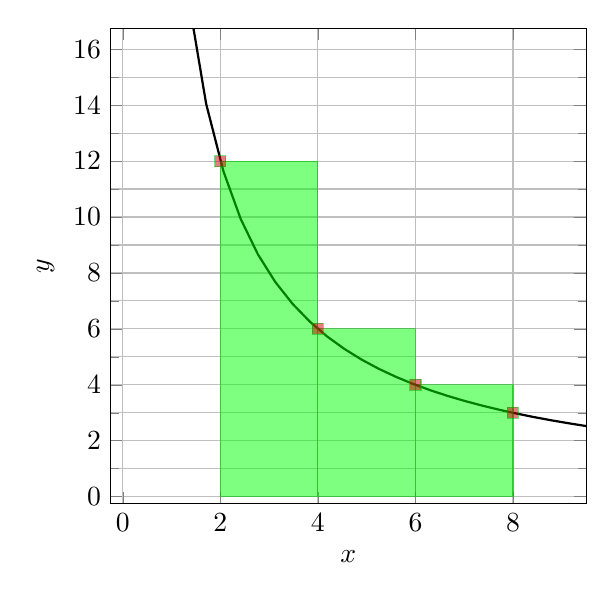
\begin{tikzpicture}
            \begin{axis}[
                xlabel = $x$,
                ylabel = $y$,
                ylabel style={rotate=90},
                xmin = -0.25, xmax = 9.5,
                ymin = -0.25, ymax = 16.75,
                grid = both,
                xtick = {0,2,4,6,8},
                ytick = {0,2,4,6,8,10,12,14,16,18},
                minor y tick num = 1,
                minor x tick num = 0,
                width = 3in,
                height = 3in,
                ylabel style={rotate=-90}]
            ]
            \addplot[ thick,black,domain=1:9.5]{24/x};

            \addplot+[ybar interval, fill=green, opacity=0.5,
            draw=green!70!black] coordinates 
            {
               (2, 12)  (4, 6) (6,4) (8,3)
            };
            
            \end{axis}
        \end{tikzpicture}
        }
    \end{center}
\end{minipage}
\vfill
\begin{minipage}{0.45\textwidth} 
\probonly{
\vspace{-140pt}
\item Now compute $R_3$, the right-hand sum using three rectangles of equal width, as an approximation of this area. Draw in these rectangles on the graph to the right.
}
\solonly{
\vspace{-70pt}
\item Now compute $R_3$, the right-hand sum using three rectangles of equal width, as an approximation of this area. Draw in these rectangles on the graph to the right.\newline
\vspace{0.5cm}

    \textbf{Solution.} $R_3$ approximates the goal area as the sum of the areas of three rectangles, whose heights correspond to $f(4)$, $f(6)$, and $f(8)$, respectively. These rectangles have a width of 2, so $R_3=2\cdot f(4)+2\cdot f(6)+2\cdot f(8)=2\cdot6+2\cdot4+2\cdot3=26$. 
}

\end{minipage}
\begin{minipage}{0.6\textwidth} \vspace{-8pt}
    \begin{center}
        \begin{tikzpicture}
            \begin{axis}[
                xlabel = $x$,
                ylabel = $y$,
                xmin = -0.25, xmax = 9.5,
                ymin = -0.25, ymax = 16.75,
                grid = both,
                xtick = {0,2,4,6,8},
                ytick = {0,2,4,6,8,10,12,14,16,18},
                minor y tick num = 1,
                minor x tick num = 0,
                width = 3in,
                height = 3in,
                ylabel style={rotate=0}]
            ]
            \addplot[name path=f, thick,black,domain=1:9.5]{24/x};
    \solonly{
            \addplot+[ybar interval, fill=red, opacity=0.5,
            draw=red!70!black] coordinates 
            {
               (2, 6)  (4, 4) (6,3) (8,3)
            }};
            \end{axis}
        \end{tikzpicture}
    \end{center}
\end{minipage}
\vfill
\item Let $A$ be the area between $y=f(x)$ and the $x$-axis from $x=2$ to $x=8$. Using your work in parts (a) and (b), place lower and upper bounds on the area $A$.
\vspace{-0.4cm}
\begin{center}
 \[
        {\fitb{1in}{\solonly{\textcolor{red}{26}}}} 
        \hspace{6pt} \leq \hspace{6pt}
        {A}
   \hspace{6pt} \leq \hspace{6pt}
        {\fitb{1in}{\textcolor{red}{44}}}
\]
\end{center}
\vspace{-0.4cm}
\vfill
\item It turns out that $A=24\ln 4 \approx33.271$. Is this consistent with your answer to (c)? How could you improve the strategy from (a) and (b) to better approximate $A$?

\begin{solution}
    Yes, the answer is consistent because the exact value of $A$ falls between 26 and 44, our computed values of $R_3$ and $L_3$, respectively. We could narrow our bounds to be closer to the exact value of $A$ by using more rectangles of smaller, equal widths.
\end{solution}

\vfill \vfill 
    \end{enumerate}
 
\newpage
 \item A car slams on its breaks and comes to a halt.  Its velocity at times between
    $t=11$ and $t=17$ is shown in the following table.
\begin{center}
    \begin{tabular}{  | c | r  r  r  r  | } 
    \hline
      $t$ (seconds)& $11$& 13& 15& 17\\
      \hline
      rate (in ft/sec)& 40& 3& 2& 0 \\ \hline
    \end{tabular}
\end{center}
  \begin{enumerate}
    \item
      \begin{problem}
        Find a good overestimate for the total distance traveled by the car
        between $t = 11$ and $t = 17$.
      \end{problem}
      
      \begin{solution}
        For the purposes of this approximation, let's assume the car travels the same velocity over each two second interval. Because we want an overestimate, let's use the highest velocity as part of our summation. To compute the distance traveled in each of the two second intervals, multiply the respective velocities (in feet per second) by time (in seconds), which is 2 seconds for each interval.
        \newline
        \newline
        $L_3 = (2)(40)+(2)(3)+(2)(2)=90$ feet.
      \end{solution}
      \vfill 

      

    \item
      \begin{problem}
        Find a good underestimate for the total distance traveled by the car
        between $t = 11$ and $t = 17$.  
      \end{problem}

      \begin{solution}
        $R_3 = (2)(3)+(2)(2)+(2)(0)=10$ feet.
      \end{solution}
\vfill 
\end{enumerate}


\item A truck begins to speed up from rest. A device recorded the truck's velocities, but the data got lost. The data that was salvaged is reproduced below, starting from $t=0$.
\begin{center}
    \begin{tabular}{  | c | r  r  r  r  | } 
    \hline
      $t$ (seconds)& $0$& 5& 10& 15\\
      \hline
      rate (in ft/sec)& $v_0$& $v_1$& $v_2$& $v_3$ \\ \hline
    \end{tabular}
\end{center}
  \begin{enumerate}
    \item
      \begin{problem}
        Using the data above, provide an overestimate of the distance traveled by the truck
        between $t = 0$ and $t = 15$.
      \end{problem}
      
        \begin{solution}
        The truck's velocity increases over time. So, to overestimate distance traveled, let's include the final, highest velocity:
        $R_3 = (5)(v_1)+(5)(v_2)+(5)(v_3)$ feet.
      \end{solution}
  \vfill 
    

    \item
      \begin{problem}
        Using the data above, provide an underestimate of the distance traveled by the truck
        between $t = 0$ and $t = 15$.
      \end{problem}
      
      \begin{solution}
        $R_3 = (5)(v_0)+(5)(v_1)+(5)(v_2)$ feet.
      \end{solution}
\vfill

\newpage

\item In reality, the truck drove for 10 minutes. Its velocities were recorded for the entire 10 minutes, in five second intervals, represented in the table below.
\begin{center}
    \begin{tabular}{  | c | r  r  r  r  r  r  | } 
    \hline
      $t$ (seconds)& $0$& 5& 10& 15&  ... &600\\
      \hline
      rate (in ft/sec)& $v_0$& $v_1$& $v_2$& $v_3$& ...& $v_{120}$ \\ \hline
    \end{tabular}
\end{center}

Write a sum that approximates the truck's total distance traveled using the data above. Your sum can include three initial terms, a final term,  as well as ... notation for unknown data points. 

\begin{solution}
    $(5)(v_1)+(5)(v_2)+(5)(v_3)+...+(5)(v_{120})$ \newline 
\newline
or $(5)(v_0)+(5)(v_1)+(5)(v_2)+...+(5)(v_{119})$
\end{solution}
  \vfill 
\begin{framed}
\begin{center} \textbf{Sigma Notation}
\end{center}

  If you wanted to calculate a sum
  using, say, 120 sub-intervals, it would be time consuming.  Sigma notation is a short cut for writing sums.  Let's look at an
  example for the problem above:
  \[ \sum_{k=0}^{119} v_k\cdot 5\]
  Here's how you read the notation:
  \begin{itemize}
  \item $\sum$ is the Greek letter Sigma; in math, it's shorthand for
    ``sum'' so you're adding a list.
  \item The $v_k\cdot 5$ to the right of the $\sum$ indicates that the terms being added up all have the form $v_k\cdot5$. %; that is, you're adding up
  %  perfect squares.
  \item The $k = 0$ below the $\sum$ and the $119$ above the $\sum$ tell you
    that $v_k$ goes from $v_0$ to $v_{119}$.  In sigma notation, the variable is
    always an integer, so in this sum $k$ will be $0$, $1$, $2$, $3$, up to $119$.
  \item Putting this all together, the notation above is shorthand for
    writing \newline 
    $v_0\cdot5 + v_1\cdot5 + v_2\cdot5 + v_3\cdot5 + ... +v_{119}\cdot5$.
  \end{itemize}
  Note:
  \begin{itemize}
      \item The letter $k$ was not important.  Consider this example:
    $\displaystyle \sum_{j=3}^7 j^2$ or $\displaystyle
    \sum_{\clubsuit=3}^7 \clubsuit^2$. These sums also equal $3^2 +
    4^2 + 5^2 + 6^2 + 7^2$.
  Here's one more example:
  \[ \sum_{n=2}^6 \frac{1}{n} = \frac{1}{2} + \frac{1}{3} + \frac{1}{4} +
  \frac{1}{5} + \frac{1}{6}.\]
 \end{itemize}
\end{framed}\newpage
\item Besides the example $\displaystyle \sum_{k=0}^{119} v_k\cdot5$ provided in the box on the previous page, the truck's total distance traveled can also be approximated as $\displaystyle \sum_{k=1}^{120} v_{k-1}\cdot5$. Can you think of other sums that are good approximations for the truck's total distance traveled? 

\begin{solution}
Examples of other reasonable sums include $\displaystyle \sum_{k=0}^{119} v_{k+1}\cdot5$ or $\displaystyle \sum_{k=1}^{120} v_{k}\cdot5$. 
\end{solution}
\vfill 
\end{enumerate}




  
%\begin{multicols}{2}

  \item
    Evaluate the following sums.
    \begin{enumerate}
    \item
      \begin{problem}
        $\displaystyle \sum_{k=1}^4 (2k+1)=$
      \end{problem}\vfill
    \begin{solution}
        $3+5+7+9=24$
      \end{solution}

    \item
      \begin{problem}
        $\displaystyle \sum_{k=1}^5 2k = $
      \end{problem}\vfill
      \begin{solution}
        $2+4+6+8+10=30$
      \end{solution}

\begin{comment}
    \item
      \begin{problem}
        $\displaystyle \sum_{k=-5}^4 k^3$
      \end{problem}
      \begin{solution}
        $-125$
      \end{solution}
\end{comment}
%\end{multicols}

    \end{enumerate}
%\newpage
  \item Put the following sums in sigma notation. 
\begin{workshop}
    It can be more challenging to convert sums to their sigma notation representations. Helpful strategies for condensing sums into sigma notation include asking: ``What stays the same in each term in the sum? What differs?"
\end{workshop}
    \begin{enumerate}
    \item
      \begin{problem}
        $ 2^4 + 3^4 + 4^4 + 5^4 = $
      \end{problem}\vfill

      \begin{solution}
        $\displaystyle \sum_{k=2}^5 k^4$ is one possible answer.  Remember
        that the variable you use in $\sum$ notation doesn't mean anything,
        so you could also write $\displaystyle \sum_{n=2}^5 n^4$.
      \end{solution}

    \item
      \begin{problem}
        $ \ln 1 + \ln 3 + \ln 5 + \ln 7 + \ln 9 + \ln 11 = $
      \end{problem}\vfill

      \begin{solution}
        $\displaystyle \sum_{k=0}^5 \ln(2k+1)$ is one possible answer.
      \end{solution}



    \end{enumerate}
    \newpage
    \item A raccoon is walking in between its home and a garbage can. At $t=0$, the raccoon leaves its home and walks towards the garbage can. The raccoon turns around and walks back home once it reaches the garbage can. The graph below shows the raccoon's \textbf{velocity} over time, in miles per hour. Positive velocity corresponds to movement towards the garbage can.
\begin{workshop}
    It is worthwhile to emphasize that this is a rate graph, or a graph of velocity, NOT distance or displacement!
\end{workshop}

     \begin{center}
        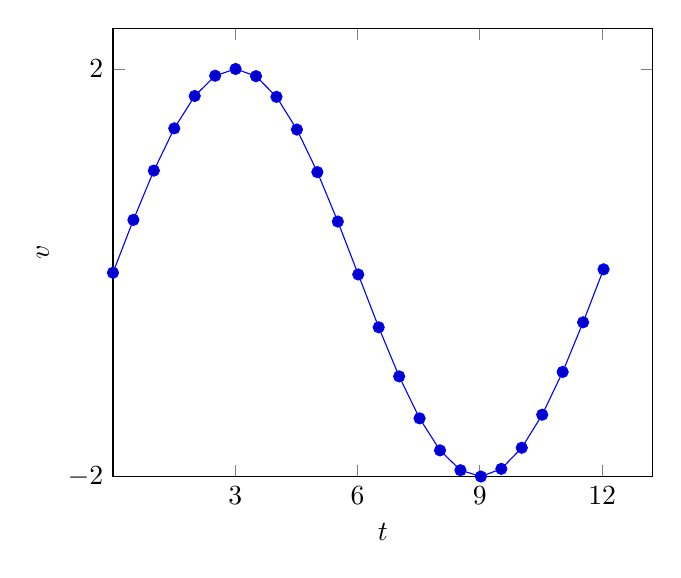
\begin{tikzpicture}
          \begin{axis}[xtick={1.57, 3.14159, 4.71, 6.28319, 9.42478, 12.5664, 15.708,
              18.8496, 21.9911, 25.1327}, xticklabels={$3$,  $6$, $9$, $12$, $
              \pi$, $4 \pi$, $5 \pi$, $6 \pi$, $7 \pi$, $8 \pi$}, xmin=0,
            ytick={-1, 1}, yticklabels={$-2$, $2$}, ymin=-1, xlabel=$t$, ylabel=$v$, ylabel style={rotate=0}] 
            \addplot+[domain=0:6.3]{sin(deg(x)};
          
          \end{axis}
        \end{tikzpicture}
      \end{center}

  
    \begin{enumerate}
        \item In what direction does the raccoon move between $t=0$ and $t=3$? Does it speed up or slow down in this interval? 
        
        \begin{solution}
        Between $t=0$ and $t=3$, the raccoon has positive velocity and therefore moves towards the garbage can. Because its velocity increases, we can say it speeds up on this interval.  
        \end{solution}
        \vfill 
        \item In what direction does the raccoon move between $t=3$ and $t=6$? Does it speed up or slow down in this interval? 

        \begin{solution}
        Between $t=3$ and $t=6$, the raccoon has positive velocity and therefore moves towards the garbage can.  Because velocity decreases, we can say it slows down on this interval.
        \end{solution}
        \vfill 
        \item When does the raccoon reach the garbage can? 
        
        \begin{solution}
        We are told that once the raccoon reaches the garbage can, it turns around and goes home. Velocity changes from positive to negative at $t=6$.  
        \end{solution}
        \vfill
        \item When is the raccoon moving the fastest towards the garbage can? Towards its home?  

        \begin{solution}
            The raccoon moves fastest towards the garbage can when the magnitude of its velocity is maximal between $t=0$ and $t=6$, which is at $t=3$. The raccoon moves fastest towards its home when the magnitude of its velocity is maximal between $t=6$ and $t=12$, which is at $t=9$. 
        \end{solution}
        \vfill 
        \item The raccoon reaches its house at $t=12$. As the raccoon closely approaches its house, does the raccoon speed up or slow down? 
        
        \begin{solution}
            The raccoon slows down as it approaches its home. We can see that the magnitude of the velocity decreases on the interval from $t=9$ to $t=12$.
        \end{solution}\vfill 
        
   

    \end{enumerate}
    \newpage
\item Suppose that, later, the same raccoon leaves its home again. Unfortunately, it loses its sense of direction and never finds the garbage can. The raccoon's velocity in miles per hour is given by the graph below. Recall that positive velocity corresponds to the raccoon moving away from its home.

 \begin{center}
        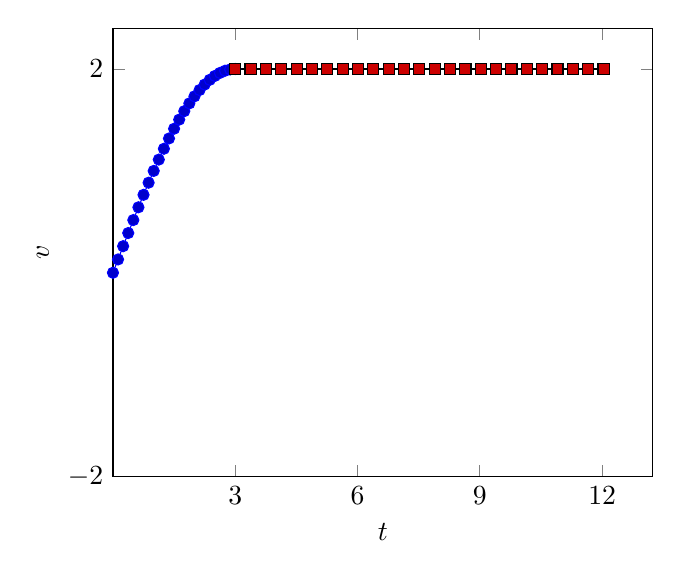
\begin{tikzpicture}
          \begin{axis}[xtick={1.57, 3.14159, 4.71, 6.28319, 9.42478, 12.5664, 15.708,
              18.8496, 21.9911, 25.1327}, xticklabels={$3$,  $6$, $9$, $12$, $
              \pi$, $4 \pi$, $5 \pi$, $6 \pi$, $7 \pi$, $8 \pi$}, xmin=0,
            ytick={-1, 1}, yticklabels={$-2$, $2$}, ymin=-1, xlabel=$t$, ylabel=$v$, ylabel style={rotate=0}] 
            \addplot+[domain=0:1.57]{sin(deg(x)};
            \addplot+[color=black][domain=1.57:6.3]{1};
          
          \end{axis}
        \end{tikzpicture}
      \end{center}

\begin{enumerate}
\item Describe the raccoon's movement between $t=3$ and $t=12$. 

\begin{solution}
    The raccoon moves at a constant velocity away from its home from $t=3$ to $t=12$.
\end{solution}
\vfill 
\item How many miles did the raccoon travel between $t=3$ and $t=12$? (Can you visualize how to calculate this distance geometrically, using the graph?)

\begin{solution}
    The raccoon travels 18 miles in the 9 hours, because it moves 2 miles per hour. This distance can be visualized as the area under the velocity graph from $t=3$ to $t=12$, which is a rectangle of length 9 and height 2.
\end{solution}
\vfill \vfill
\item \textit{Exploratory} How would you \textbf{approximate} the distance that the raccoon travels between $t=0$ and $t=12$? (Can you visualize how to \textbf{approximate} this distance geometrically on the graph?)

\begin{solution}
    Using a similar strategy to visualize area under the velocity graph from $t=0$ to $t=3$, we could approximate this area as a triangle with length 3 and height 2. The area of this triangle would be $\frac{1}{2}\cdot3\cdot2=3$. Thus, the raccoon would have traveled about 3 miles from $t=0$ to $t=3$.
\end{solution}
\vfill \vfill
\end{enumerate}
%\newpage
%\item \textit{Limits Challenge!} Compute the following challenge limits.
%\begin{enumerate}
%    \item $\displaystyle \lim_{x \to 1^{-}}\dfrac{\arccos x}{\ln x}$
%    \vfill
%    \item $\displaystyle \lim_{x \to 0^{+}}\dfrac{\ln x}{\tan \left({x+\dfrac{\pi}{2}}\right)}$
%    \vfill
%    \item $\displaystyle \lim_{x \to 0^{-}}x^{-2}\arcsin x$
%    \vfill
%    \item $\displaystyle \lim_{x \to \infty} \left(\dfrac{x}{x+1}\right)^x$
%    \vfill
%    \vfill
%\end{enumerate}
\end{enumerate}
\end{document}
